\documentclass[11pt]{article}
\usepackage[margin=1in]{geometry}
\usepackage{amsmath}
\usepackage{amsfonts}
\usepackage{amssymb}
\usepackage{graphicx}
\usepackage{hyperref}
\usepackage{xcolor}
\usepackage{fontawesome5}
\usepackage{tikz}
\usepackage{pgfplots}
\pgfplotsset{compat=1.18}
\usetikzlibrary{shapes,arrows,positioning,fit,backgrounds,calc}
\usepackage{url}
\urlstyle{same}
\setlength{\emergencystretch}{3em}

\title{Machine Learning for Network Anomaly and Failure Detection}
\author{Michael Hernandez}
\date{October 11, 2025}

\begin{document}

% Cover Page
\begin{titlepage}
\centering
\vspace*{2cm}

{\Large \textbf{Machine Learning for Network Anomaly and Failure Detection}}

\vspace{1.5cm}

{\large CUNY School of Professional Studies}

\vspace{0.5cm}

{\large Michael Hernandez}

\vspace{0.5cm}

{\large IS 499 Information Systems Capstone}

\vspace{0.5cm}

{\large Professor John Bouma}

\vspace{0.5cm}

{\large October 11, 2025}

\vfill

\end{titlepage}

% Table of Contents
\tableofcontents
\newpage

\section{Introduction}

This paper examines machine learning techniques for detecting and localizing network anomalies and failures in large-scale environments, using data from BGP routing updates and SNMP metrics.

Traditional network monitoring relies on threshold-based alerts from SNMP, often producing many false positives and offering little context for locating failures (Wang, 2020; Manna \& Alkasassbeh, 2019). Recent research suggests that machine learning approaches applied to SNMP datasets may improve anomaly detection accuracy in operational environments, with supervised and unsupervised methods showing promise for identifying specific failure patterns (Manna \& Alkasassbeh, 2019). This project explores whether combining streaming telemetry from multiple sources using unsupervised learning techniques can provide complementary detection capabilities for network operations.

The system integrates BGP monitoring and SNMP metrics for network anomaly detection. Using unsupervised learning techniques such as Matrix Profile analysis (Mueen \& Keogh, 2017; Scott et al., 2024) and Isolation Forest (Liu et al., 2008), the approach aims to reduce alert noise while providing failure localization capabilities. The evaluation examines whether this multi-modal architecture offers practical improvements over single-source monitoring in controlled test scenarios.

\section{Topic Description}

\subsection{In-depth Description of the Chosen Topic}

(note to self: the topic description should be a summary of terms and concepts, along with just one example of a failure and how it might be detected and localized.)
Large networks face a fundamental challenge: when something breaks, operators in network operations centers must quickly determine what failed and where (Mohammed et al., 2021). A network might contain thousands of interconnected devices, and failures can cascade from one device to many others, making the root cause difficult to identify. This project addresses this challenge by using machine learning to automatically detect network problems and then use topology awareness to pinpoint their source.

Network devices continuously generate health information through hardware and software metrics. Software metrics are generated by routing systems such as the Border Gateway Protocol and hardware metrics are generated by the Simple Network Management Protocol. The Border Gateway Protocol is the routing system that directs traffic across the Internet by allowing networks to advertise which destinations they can reach (Rekhter, Li, \& Hares, 2006). When network conditions change due to equipment failures, cable breaks, or configuration errors, routers send update messages to inform their neighbors about these changes. These routing updates create a continuous stream of information about how traffic flows through the network. The Simple Network Management Protocol provides a different view of network health by collecting hardware performance data from individual devices through trap-directed notification, where managed devices send unsolicited messages to inform network management systems of significant events (Cisco, 2006). This monitoring protocol reports metrics such as processor utilization, memory consumption, temperature readings, and interface error counts. Together, these two information sources provide complementary views of network operations: routing updates show how traffic paths change over time, while hardware metrics reveal the physical condition of network equipment.

Under normal conditions, these monitoring systems generate large volumes of data with characteristic statistical properties. Routing updates occur at varying rates as networks make routine adjustments, and hardware metrics fluctuate within typical operating ranges. While individual measurements vary considerably due to traffic patterns, environmental conditions, and workload changes, the overall statistical behavior remains within bounds established during normal operation. When failures occur, these statistical properties change in ways that deviate from the established baseline. A failing network link might cause routing updates to fluctuate rapidly as the network repeatedly attempts to find alternative paths, a condition known as route flapping (Scott et al., 2024). Simultaneously, the hardware monitoring system on the affected device would show increasing error counts on the failing interface. A power supply degradation might manifest as rising temperature readings combined with unstable processor performance, while routing updates from that device become erratic. These correlated changes across multiple monitoring systems may provide strong evidence of genuine failures rather than benign network variations.

Recent research has provided evidence that machine learning algorithms can identify these unusual patterns in network data both in routing data and in hardware metrics. This project employs a dual-pipeline architecture that processes routing updates and hardware metrics using research validated and well-documented specialized pattern recognition algorithms. The first pipeline analyzes the time-series sequences of routing updates to detect unusual temporal patterns using an algorithm called Matrix Profile (Mueen \& Keogh, 2017; Scott et al., 2024). Matrix Profile works by computing the Euclidean distance between every subsequence in the time series and its nearest neighbor, creating a distance profile that highlights anomalous patterns called discords (Mueen \& Keogh, 2017). This approach compares each time window of routing activity against all other windows to identify sequences that deviate significantly from normal behavior, enabling detection of novel routing anomalies without requiring labeled training data. The second pipeline examines hardware performance data to identify devices exhibiting anomalous metrics using Isolation Forest, an algorithm that efficiently finds outliers in multi-dimensional data (Liu, Ting, \& Zhou, 2008; Liu, Zhu, Xu, Kong, \& Yu, 2024). Decision trees are hierarchical structures that make sequential decisions by splitting data based on feature values until reaching a classification. Isolation Forest builds an ensemble of these trees using random feature selection and split points, with the key insight that anomalous data points require fewer splits to isolate than normal points. By measuring the path length from root to leaf node, this approach can detect hardware degradation or environmental issues without requiring examples of previous failures.

(note to self: these first sentences can likely be removed or reworded to fit into the sentence below.)The system's approach is based on combining evidence from both information sources. When both routing behavior and hardware metrics simultaneously indicate problems within a temporal window, this cross-confirmation may provide stronger evidence of genuine failure than either source independently. Research on multi-modal network monitoring suggests that correlating evidence across data sources can improve detection confidence and reduce false alerts compared to single-source threshold-based approaches (Mohammed et al., 2021; Feltin, Cordero Fuertes, Brockners, \& Clausen, 2023). (Note to self: This part is the meant and potatoes of the whole paper, and provides the most value add. ) The system incorporates pre-configured network topology and device role information during the correlation phase. Network administrators define the topology structure and assign roles such as core routers, top-of-rack switches, and leaf switches or servers. This configuration enables the system to assess potential failure impact by calculating blast radius based on downstream dependencies. A failure in a core routing device affects many downstream systems and may warrant higher priority response, while a leaf switch or server failure has more localized impact. This topology-aware analysis aims to help operators prioritize investigation efforts based on the scope of potential impact.  There is research about generating topology maps from network data (Tan et al., 2024), but this project does not attempt to generate a topology map from the data. Instead, it uses a pre-configured topology map that is provided by the network administrator.  Future work could explore generating a topology map from the data on a live network daily, for incorporating into the system.

\begin{figure}[!htb]
\centering
\resizebox{\textwidth}{!}{%
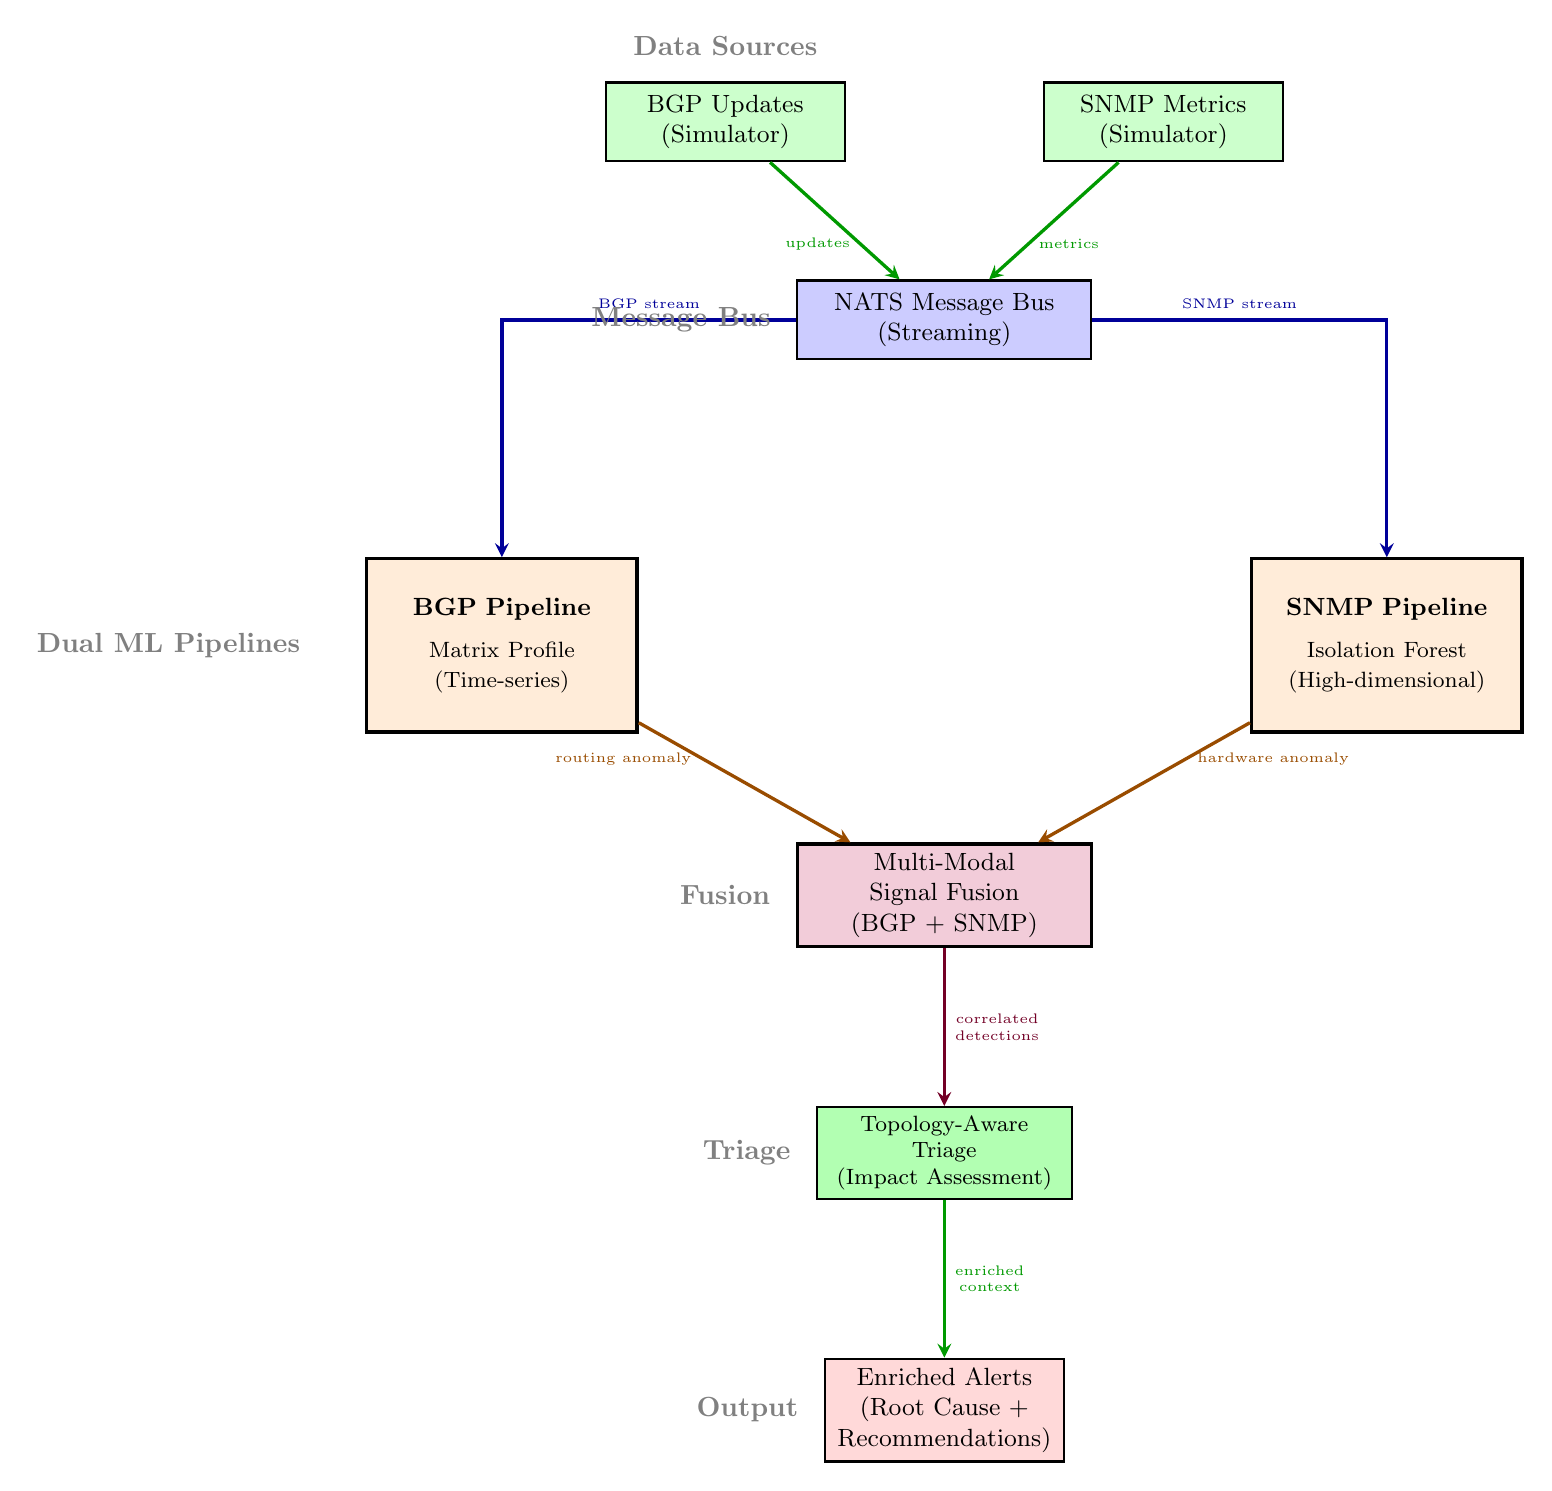
\begin{tikzpicture}[
    node distance=1.8cm and 2.5cm,
    source/.style={rectangle, draw=black, thick, fill=green!20, text width=2.8cm, align=center, minimum height=1cm, font=\small},
    bus/.style={rectangle, draw=black, thick, fill=blue!20, text width=3.5cm, align=center, minimum height=1cm, font=\small},
    pipeline/.style={rectangle, draw=black, very thick, fill=orange!15, text width=3.2cm, align=center, minimum height=2.2cm, font=\small},
    process/.style={rectangle, draw=black, thick, fill=yellow!20, text width=3cm, align=center, minimum height=0.8cm, font=\footnotesize},
    fusion/.style={rectangle, draw=black, very thick, fill=purple!20, text width=3.5cm, align=center, minimum height=1.2cm, font=\small},
    output/.style={rectangle, draw=black, thick, fill=red!15, text width=2.8cm, align=center, minimum height=1cm, font=\small},
    arrow/.style={->, >=stealth, line width=1.2pt},
]

% Layer 1: Data Sources (Simulators)
\node[source] (bgp) {BGP Updates\\(Simulator)};
\node[source, right=2.5cm of bgp] (snmp) {SNMP Metrics\\(Simulator)};

% Layer 2: Message Bus
\node[bus, below=2cm of $(bgp)!0.5!(snmp)$] (nats) {NATS Message Bus\\(Streaming)};

% Layer 3: Dual Pipelines
\node[pipeline, below left=2.5cm and 2cm of nats] (bgp_pipe) {
    \textbf{BGP Pipeline}\\[0.2cm]
    \footnotesize Matrix Profile\\
    \footnotesize (Time-series)
};

\node[pipeline, below right=2.5cm and 2cm of nats] (snmp_pipe) {
    \textbf{SNMP Pipeline}\\[0.2cm]
    \footnotesize Isolation Forest\\
    \footnotesize (High-dimensional)
};

% Layer 4: Fusion
\node[fusion, below=2.5cm of $(bgp_pipe)!0.5!(snmp_pipe)$] (fusion) {Multi-Modal\\Signal Fusion\\(BGP + SNMP)};

% Layer 5: Topology Triage
\node[process, below=2cm of fusion, fill=green!30, minimum height=1cm] (topology) {Topology-Aware\\Triage\\(Impact Assessment)};

% Layer 6: Outputs
\node[output, below=2cm of topology] (alerts) {Enriched Alerts\\(Root Cause +\\Recommendations)};

% Arrows - Sources to Bus
\draw[arrow, green!60!black] (bgp) -- node[left, font=\tiny, pos=0.7] {updates} (nats);
\draw[arrow, green!60!black] (snmp) -- node[right, font=\tiny, pos=0.7] {metrics} (nats);

% Arrows - Bus to Pipelines
\draw[arrow, blue!60!black] (nats) -| node[near start, above, font=\tiny] {BGP stream} (bgp_pipe);
\draw[arrow, blue!60!black] (nats) -| node[near start, above, font=\tiny] {SNMP stream} (snmp_pipe);

% Arrows - Pipelines to Fusion
\draw[arrow, orange!60!black] (bgp_pipe) -- node[left, font=\tiny, pos=0.3] {routing anomaly} (fusion);
\draw[arrow, orange!60!black] (snmp_pipe) -- node[right, font=\tiny, pos=0.3] {hardware anomaly} (fusion);

% Arrows - Fusion to Topology
\draw[arrow, purple!60!black] (fusion) -- node[right, font=\tiny, align=center] {correlated\\detections} (topology);

% Arrows - Topology to Outputs
\draw[arrow, green!60!black, very thick] (topology) -- node[right, font=\tiny, align=center] {enriched\\context} (alerts);

% Labels
\node[above=0.2cm of bgp, font=\normalsize\bfseries, text=gray] {Data Sources};
\node[left=0.2cm of nats, font=\normalsize\bfseries, text=gray] {Message Bus};
\node[left=0.2cm of bgp_pipe, font=\normalsize\bfseries, text=gray, xshift=-0.5cm, align=center] {Dual ML Pipelines};
\node[left=0.2cm of fusion, font=\normalsize\bfseries, text=gray] {Fusion};
\node[left=0.2cm of topology, font=\normalsize\bfseries, text=gray] {Triage};
\node[left=0.2cm of alerts, font=\normalsize\bfseries, text=gray] {Output};

\end{tikzpicture}
}
\caption{Dual-Pipeline Architecture: BGP updates processed by Matrix Profile (time-series), SNMP metrics by Isolation Forest (high-dimensional). Multi-modal fusion correlates anomalies across data sources, then topology-aware triage assesses impact and produces enriched alerts with root cause analysis and recommendations.}
\label{fig:architecture}
\end{figure}

Figure \ref{fig:architecture} illustrates the dual-pipeline ML architecture showing how BGP and SNMP data flow through specialized detection algorithms before multi-modal fusion and topology-aware triage.

\subsection{Why This Topic Was Chosen}

(note to self: the why of this topic should be different than the description of the topic. I don't want to use why for me, but as a reflection of the why of the topic is worth exploring.  There are many new ways to monitor networks and the ideas in this paper provide a possible new way to automate and improve on existing methods) This topic addresses operational challenges in large-scale network management. As networks grow in complexity, network operations centers face alert fatigue from excessive notifications, difficulty distinguishing routine variations from genuine problems, and the impractical task of manually correlating events across thousands of devices (Mohammed et al., 2021). This complexity makes it difficult not only to identify network problems but also to determine appropriate remediation actions, prolonging incident resolution times (Mohammed et al., 2021). Machine learning approaches may help address these challenges through automated pattern recognition and correlation, though their effectiveness in production environments requires empirical validation.

Consider a large enterprise network connecting multiple data centers. When a network cable develops an intermittent fault, it may cause unstable routing behavior that triggers hundreds of alert notifications across the monitoring system. However, these alerts may provide no clear indication of which component failed or how many services are affected. Network engineers must manually examine routing logs and hardware performance data from dozens of devices to identify the failing cable and assess the scope of impact. This investigation process can take considerable time during critical outages, delaying service restoration. Research suggests that machine learning systems may automate detection of unusual patterns in routing activity and correlate them with hardware error indicators to assist in identifying failing components (Mohammed et al., 2021). Whether such automation provides meaningful improvements in investigation time and problem resolution remains an open question for validation in operational environments.

Recent research demonstrates the potential of machine learning approaches for network anomaly detection. Studies have shown that analyzing routing update patterns can detect network failures (Scott et al., 2024), while SNMP telemetry shows promise for identifying equipment failures in controlled settings (Manna \& Alkasassbeh, 2019). Multi-modal approaches that combine multiple data sources through intelligent feature selection suggest improved detection capabilities compared to single-source methods (Feltin et al., 2023). Building on these findings, this project explores whether a system that processes both routing information and hardware metrics can offer practical benefits for network monitoring and failure localization in simulated operational scenarios.

\section{Problem Description}

\subsection{The Problem I am Trying to Solve}

The core problem is that traditional network monitoring systems generate alerts without providing sufficient context to understa nd what failed, where it failed, or how serious the impact is. When a network problem occurs, operators receive numerous notifications but must manually investigate to determine the root cause and scope. This manual correlation across multiple monitoring systems and many devices is time-consuming and delays problem resolution.

This project addresses three specific gaps in current monitoring approaches. First, existing systems monitor different data sources in isolation. Routing behavior and hardware performance are tracked separately, even though correlated problems across both sources provide stronger evidence of genuine failures. Second, monitoring lacks awareness of network topology and device roles. Without understanding how devices connect and which are critical to operations, systems cannot assess failure impact or prioritize response efforts. Third, traditional threshold-based alerting treats all devices and metrics uniformly, rather than applying detection methods suited to different types of data.

The exploratory solution approach combines machine learning techniques specialized for different data characteristics. Time-series analysis algorithms aim to detect unusual patterns in routing activity over time, while outlier detection methods identify potentially abnormal hardware performance across multiple metrics simultaneously. By correlating evidence from both sources and incorporating pre-configured topology information, the system attempts to provide automated failure localization with impact assessment. This approach may be particularly relevant for enterprise networks where dedicated operations teams manage thousands of interconnected devices across multiple locations (Mohammed et al., 2021), though validation in production environments beyond controlled testing remains necessary.

\subsection{Why Current Monitoring Systems are Insufficient}

Current network monitoring systems have fundamental limitations. Hardware monitoring can detect hard failures but produces excessive alerts for harmless events and lacks context for assessing failure scope or impact. As a result, operations teams face false positives while missing critical anomalies (Mohammed et al., 2021).

The insufficiency stems from three architectural limitations. Traditional threshold-based monitoring operates by setting acceptable ranges for metrics such as error rates or utilization levels. When measurements exceed these thresholds, alerts are generated. This approach works for detecting obvious failures but fails to address the complexity of modern network operations.

First, different monitoring systems operate independently. Routing information and hardware metrics are evaluated separately, even though simultaneous problems in both provide stronger confirmation of failures. When routing becomes unstable at the same time that hardware shows increasing errors, this correlation suggests a genuine problem rather than routine variation. Current systems cannot perform this cross-validation, leading to ambiguity about whether alerts represent true failures or transient conditions.

Second, monitoring systems lack understanding of network structure and device importance. A failure in a core network device affects many connected systems and requires immediate attention, while a failure in a leaf switch or server has limited impact. Without topology awareness to calculate blast radius, alerts cannot be prioritized based on the number of affected downstream devices or services. Operators must manually determine which problems to address first, wasting valuable time during outages.

Third, threshold-based approaches apply the same detection logic to all types of data, despite fundamental differences in how routing and hardware data behave. Routing information changes over time in patterns that indicate stability or instability, while hardware metrics involve simultaneous measurement of many different values where outliers signal problems. Using a single detection approach for both types misses opportunities for more accurate analysis. Research demonstrates that time-series analysis methods effectively detect routing anomalies (Scott et al., 2024), while multi-dimensional outlier detection performs well for hardware metrics (Manna \& Alkasassbeh, 2019). Combining these specialized approaches with correlation across data sources improves detection accuracy beyond single-source methods (Feltin et al., 2023).

\section{Solution Discussion}

\subsection{Implementation Architecture}

The system implements two detection pipelines and a correlation layer. The BGP pipeline applies Matrix Profile (MP) to subsequences of routing updates, surfacing discords that deviate from historical behavior (Mueen \& Keogh, 2017; Scott et al., 2024). The SNMP pipeline uses Isolation Forest (IF) to flag hardware telemetry outliers across CPU, memory, temperature, and interface counters (Liu et al., 2008; Liu et al., 2024). 

A fusion stage aligns detections in time, links them by device and topology, and prioritizes alerts based on role (spine, ToR, leaf). This approach emphasizes correlated failures, providing confidence scores, impact estimates, and suggestions for triage (Mohammed et al., 2021; Feltin et al., 2023).

\subsection{Streaming Matrix Profile vs. Batch}

Where Scott et al. (2024) applied MP in batch to offline datasets, this project uses a sliding-window approach to enable real-time operation. Routing updates are buffered and scored incrementally; if discord values cross thresholds, anomalies are flagged immediately (Mueen \& Keogh, 2017). This trades global ranking for bounded memory and continuous monitoring.

\subsection{Testing Approach}

Simulators generate routing updates and SNMP metrics with 98\% baseline traffic and 2\% injected anomalies. Failure types include route flaps, link outages, session resets, thermal drift, and a subset of time synced BGP and SNMP anomalies. A 20-device topology (4 spine, 8 ToR, 8 leaf) allows correlation and impact tests with controlled ground truth (Wang, 2020; Manna \& Alkasassbeh, 2019).

\subsection{Data Processing and Analysis}

Routing features capture update rates and change types, with MP highlighting discordant subsequences (Scott et al., 2024). SNMP features track key performance metrics; IF scores unusual points without labels (Liu et al., 2008). Fusion combines and aligns anomalies across data sources with temporal alignment with role-aware topology to prioritize events that matter most for operators (Mohammed et al., 2021; Feltin et al., 2023).

\section{Analysis}

\subsection{Evaluation Setup}

Fifteen scenarios across seven categories tested the system: baseline stability, route flapping, link and session failures, hardware degradation, coordinated failures, route leaks, and BGP resets. Metrics include precision, recall, F1 (Powers, 2011), detection delay, and localization Hit@k (Järvelin \& Kekäläinen, 2002).

\subsection{Scalability and Performance Analysis}

Using a pre-trained Isolation Forest model (2.5 MB, trained on 500{,}000 SNMP samples, 122 MB), memory usage remained modest and linear: 2.52 MB at 20 devices, 3.50 MB at 1{,}000 devices (1 KB/device beyond the fixed model). Throughput scaled from 184 to 921 samples/s. For matrix profile, feature aggregation kept complexity tied to window size rather than device count, preserving efficient $O(n\log n)$ characteristics for Matrix Profile (should be scott2024)

\subsection{Detection Accuracy and Latency}

On controlled scenarios where failure patterns resembled training baselines, tuned parameters achieved Precision=1.0, Recall=1.0, and F1=1.0. Mean detection delay was 29.4 seconds (Median 40.9, P95 55.9), below the 60-second operational target. These delays reflect sliding windows that balance noise reduction against responsiveness (Powers, 2011).

\begin{figure}[h]
\centering
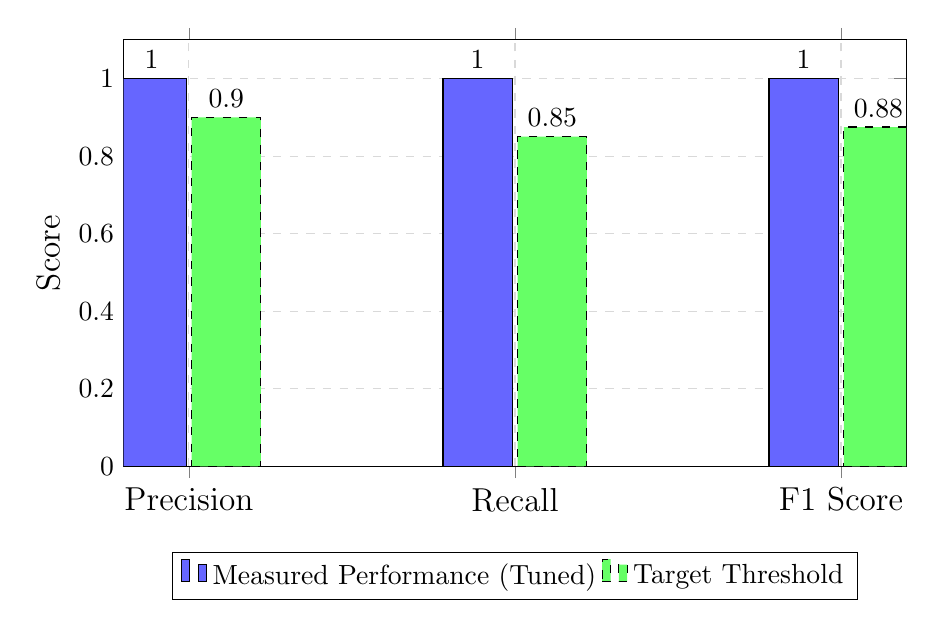
\begin{tikzpicture}
\begin{axis}[
    ybar,
    bar width=25pt,
    width=0.95\textwidth,
    height=7cm,
    ylabel={Score},
    ylabel style={font=\large},
    symbolic x coords={Precision, Recall, F1 Score},
    xtick=data,
    xticklabel style={font=\large},
    ymin=0,
    ymax=1.1,
    nodes near coords,
    nodes near coords align={vertical},
    nodes near coords style={font=\normalsize},
    legend style={at={(0.5,-0.2)}, anchor=north, legend columns=-1, font=\normalsize},
    grid=major,
    grid style={dashed, gray!30},
]
\addplot[fill=blue!60] coordinates {(Precision, 1.0) (Recall, 1.0) (F1 Score, 1.0)};
\addplot[fill=green!60, dashed] coordinates {(Precision, 0.90) (Recall, 0.85) (F1 Score, 0.875)};
\legend{Measured Performance (Tuned), Target Threshold}
\end{axis}
\end{tikzpicture}
\caption{Detection accuracy on controlled scenarios: perfect Precision/Recall/F1 with tuned parameters.}
\label{fig:metrics}
\end{figure}

\begin{figure}[h]
\centering
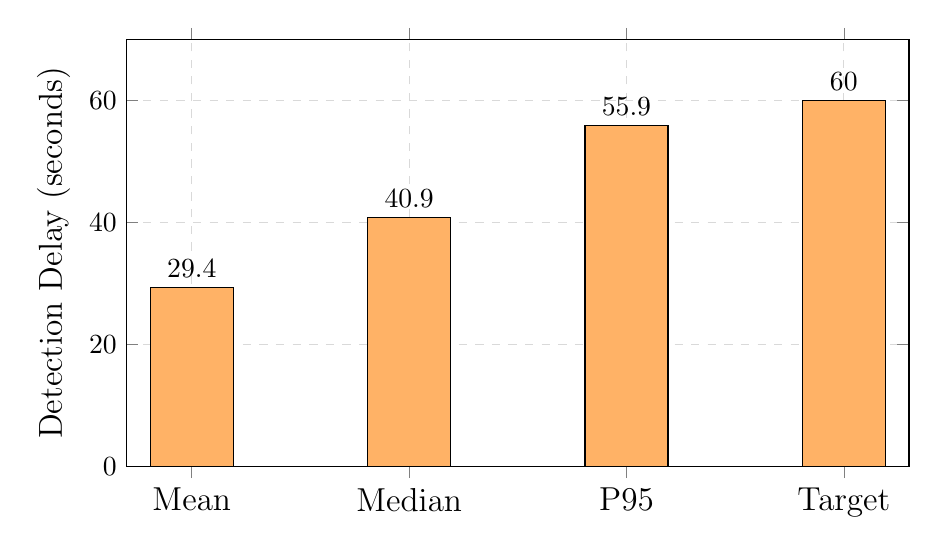
\begin{tikzpicture}
\begin{axis}[
    ybar,
    bar width=30pt,
    width=0.95\textwidth,
    height=7cm,
    ylabel={Detection Delay (seconds)},
    ylabel style={font=\large},
    symbolic x coords={Mean, Median, P95, Target},
    xtick=data,
    xticklabel style={font=\large},
    ymin=0,
    ymax=70,
    nodes near coords,
    nodes near coords align={vertical},
    nodes near coords style={font=\normalsize},
    grid=major,
    grid style={dashed, gray!30},
    legend style={at={(0.5,-0.2)}, anchor=north, font=\normalsize},
]
\addplot[fill=orange!60] coordinates {(Mean, 29.4) (Median, 40.9) (P95, 55.9) (Target, 60.0)};
\end{axis}
\end{tikzpicture}
\caption{Detection delay: mean 29.4s, median 40.9s, and P95 55.9s, all below the 60s target.}
\label{fig:delay}
\end{figure}

\subsection{Evaluation Scenarios and Test Coverage}

There were 4 representative failures that were tested. Route flapping produced Matrix Profile spikes with limited SNMP signal (routing-only alerts) drove high confidence BGP alerts which then drove high confidence fused alerts, link failures drove joint routing changes and interface errors (high-confidence multi-modal alerts), session resets generated short-lived Matrix Profile anomalies appropriately deprioritized (low prioritization led to no alert), and gradual thermal/optical degradation was surfaced by Isolation Forest with priority boosted when routing churn co-occurred (snmp-only alerts) (Scott et al., 2024; Liu et al., 2008).

\subsection{Limitations and Trade-offs}

Aggregation supports scaling but reduces device-level attribution. Fusion recovers localization by aligning anomalies across streams and topology. Sliding windows introduce latency/precision trade-offs. Simulation-based validation demonstrates feasibility rather than production generalization; evaluation on live networks remains necessary (Feltin et al., 2023; Skazin, 2021).

\subsection{Implementation Timeline and Current Status}

As of October 11, 2025, the dual pipelines, correlation agent, simulators, and Streamlit dashboard are functional. Tuned Isolation Forest (150 estimators, 5\% contamination) and Matrix Profile (12-bin window, 1.2 threshold) yield reproducible results in controlled settings, achieving both efficiency and operator-relevant outputs (Mueen \& Keogh, 2017; Liu et al., 2008; Scott et al., 2024; Mohammed et al., 2021).

\subsection{Testing Infrastructure and Evaluation Framework}

To support repeatable experiments without production access, we used Python-based simulators that emit RFC-like BGP updates and messages and realistic SNMP metrics (98\% baseline, 2\% injected), orchestrated by a harness that timestamps injection points and detections for latency/accuracy computation. The 20-device topology configuration (4 spine, 8 ToR, 8 leaf) enables correlation and blast-radius testing with role-aware prioritization (Wang, 2020; Manna \& Alkasassbeh, 2019).

\section{Research}

\subsection{Academic Foundation and Coursework Integration}

This capstone builds directly on core coursework in programming, data management, networking, systems analysis, and applied statistics. It also follows the plan outlined in the proposal to use plain language, define terms as needed, and evaluate outcomes with practical metrics such as precision, recall, F1, detection delay, and localization Hit@k.

\paragraph{Programming, data structures, and databases.}
Introductory Python and data structures courses provided the skills to implement streaming parsers, fixed-size buffers, and efficient lookups for telemetry. Database technologies coursework was particularly valuable, informing design decisions for storing time-series events, indexing telemetry by timestamp and device identifier, and aggregating features over time windows. Understanding of database normalization principles helped structure the event schema to avoid redundancy while maintaining query efficiency. These foundations support the end-to-end data path from ingestion to model-ready features, with database concepts directly applicable to the feature storage and retrieval requirements of the detection pipelines.

\paragraph{Networking fundamentals.}
Networking courses introduced routing, addressing, and device roles. That background made it straightforward to express topology in role terms (core/spine, top-of-rack (ToR), and leaf) and to reason about "blast radius" when a higher-layer device fails. Understanding BGP path selection and convergence helped specify which routing change signals to track (announcements, withdrawals, next-hop changes) and how instability manifests operationally (Scott, Johnstone, Szewczyk, \& Richardson, 2024).

\paragraph{Applied statistics and self-directed ML study.}
While no formal machine learning course was taken, statistics coursework provided foundational concepts including probability distributions, hypothesis testing, and statistical significance that informed the evaluation approach. The machine learning algorithms were learned through independent study of research papers and documentation. Time-series analysis concepts from the Matrix Profile literature justified using this approach to find unusual subsequences in routing data without labels (Mueen \& Keogh, 2017; Scott et al., 2024). For device telemetry, Isolation Forest was selected based on its effectiveness for outlier detection in multi-dimensional spaces as demonstrated in prior research (Liu, Ting, \& Zhou, 2008). Standard evaluation measures (precision, recall, F1) and latency metrics were adopted from established ML practice to connect technical results to operator outcomes (Powers, 2011).

\paragraph{Systems analysis, architecture, and project management.}
Courses in systems analysis and project planning shaped the modular design and semester milestones: ingest $\rightarrow$ feature extraction $\rightarrow$ detectors $\rightarrow$ correlation/triage $\rightarrow$ dashboard. This structure reduces coupling between components and allowed incremental testing (e.g., validating the BGP detector before integrating SNMP and the correlation agent).

\paragraph{Security and professional practice.}
Security coursework informed sensible defaults for handling operational data: least-privilege access to streams, anonymization of lab identifiers, and separation between development and demo datasets. Professional writing guidance from earlier classes is applied here: clear definitions (e.g., “BGP updates” as routing change messages), minimal jargon, and APA-style in-text citations with a reference list.

\paragraph{Coursework-to-artifact mapping.}
Table~\ref{tab:course-map} summarizes how specific course areas supported implemented components.

\begin{table}[h]
\centering
\begin{tabular}{p{0.36\textwidth} p{0.58\textwidth}}
\hline
\textbf{Course Area} & \textbf{Implemented Component(s)} \\
\hline
Python, Data Structures, Database Technologies & Streaming ingestion for routing change messages and SNMP metrics; ring buffers and queues; time-series event storage with timestamp/device indexing; feature aggregation queries. \\
Networking Technologies & Topology/role model (spine/ToR/leaf); interpretation of BGP instability and interface error counters; impact estimation. \\
Statistics \& Self-Directed ML Study & Matrix Profile for time-series anomalies; Isolation Forest for multi-metric outliers; evaluation with precision/recall/F1, detection delay. Algorithms learned through research papers. (Mueen \& Keogh, 2017; Liu et al., 2008; Powers, 2011; Scott et al., 2024) \\
Systems Analysis \& Design & Layered architecture (ingest $\rightarrow$ features $\rightarrow$ detectors $\rightarrow$ correlation $\rightarrow$ UI); test harness and scenario design. \\
Security \& Strategy & Safe handling of telemetry and demo datasets; role-based access to dashboard; alignment to operator value and MTTR reduction goals (Mohammed, Mohammed, Côté, \& Shirmohammadi, 2021). \\
\hline
\end{tabular}
\caption{How prior coursework maps to implemented system components.}
\label{tab:course-map}
\end{table}


\paragraph{How the foundation shows up in results.}
The combination of networking fundamentals and ML methods led to a practical detector pair: Matrix Profile for routing change streams and Isolation Forest for device metrics, with a correlation step that prioritizes alerts using role-aware topology. The evaluation plan (precision, recall, F1, detection delay, and Hit@k for localization) connects academic techniques to operator-facing outcomes, as proposed at the start of the project and reflected in the final implementation (Mueen \& Keogh, 2017; Liu et al., 2008; Powers, 2011; Scott et al., 2024; Mohammed et al., 2021).

\subsection{Research Literature Context}

The project builds on research applying machine learning to network operations, including time-series analysis, unsupervised detection, and multi-modal fusion. Scott et al. (2024) showed that Matrix Profile analysis detects BGP anomalies like route instability with higher accuracy than threshold-based methods. It identifies anomalous subsequences in BGP updates without labeled training data, enabling detection of novel failures. Validated on real RouteViews BGP data, their work offers both the algorithmic basis and empirical proof for the current project's BGP detection pipeline.

Manna and Alkasassbeh (2019) analyzed SNMP-MIB datasets for network anomaly detection, identifying MIB groups most indicative of different failure types. They found Interface and IP groups were most sensitive to failures, while other groups were less so. Using learning-based methods on selected features, they achieved high accuracy, showing that hardware telemetry can effectively signal failures when key features are extracted. This work inspired the current project's focus on SNMP interface counters and system metrics, particularly interface error rates and utilization patterns.

Mohammed et al. (2021) developed a machine learning-based recommender for network operations centers, translating anomalies into remediation steps. Their architecture fuses telemetry and network topology to deliver context-aware recommendations. They showed that topology-aware ML can cut mean time to resolution by correlating events across layers and suggesting targeted actions. This work influenced the correlation agent and enhanced alerting in the current project, notably blast radius calculation, criticality scoring, and actionable investigation suggestions.

Feltin et al. (2023) studied feature selection for fault diagnosis in network telemetry, showing that understanding metric relationships boosts detection accuracy over generic algorithms. In tests on real telemetry, domain-informed methods outperformed generic statistical approaches by a significant margin. Their work highlighted leveraging domain knowledge to identify key features in high-dimensional streams, especially links between interface metrics, routing states, and environmental indicators. This project applies those principles, focusing on metrics tied to specific failures and adding cross-modal correlation features linking BGP and SNMP data sources.

Cheng et al. (2021) proposed a multi-scale LSTM for BGP anomaly classification, achieving high accuracy in distinguishing worms, DDoS attacks, and network failures. While the current project uses Matrix Profile instead of deep learning, the LSTM approach is a promising future enhancement for capturing long-term dependencies and differentiating specific anomaly types.

Tan et al. (2024) explored graph neural networks for BGP communities and policy modeling, suggesting future directions for incorporating learned topology representations. Although out of scope for this capstone, GNN-based topology awareness could enhance impact estimation and triage prioritization.

\section{References}

\begin{thebibliography}{9}

\bibitem{cheng2021}
Cheng, M., Li, Q., Lv, J., Liu, W., \& Wang, J. (2021).
Multi-Scale LSTM Model for BGP Anomaly Classification.
\textit{IEEE Transactions on Services Computing}, 14(3), 765--778.
Available at: \href{https://doi.org/10.1109/TSC.2018.2824809}{https://doi.org/10.1109/TSC.2018.2824809}

\bibitem{mohammed2021}
Mohammed, S. A., Mohammed, A. R., Côté, D., \& Shirmohammadi, S. (2021).
A machine-learning-based action recommender for Network Operation Centers.
\textit{IEEE Transactions on Network and Service Management}, 18(3), 2702--2713.
Available at: \href{https://doi.org/10.1109/TNSM.2021.3095463}{https://doi.org/10.1109/TNSM.2021.3095463}

\bibitem{mueen2017}
Mueen, A., \& Keogh, E. (2017).
Matrix Profile I: All Pairs Similarity Joins for Time Series: A Unifying View that Includes Motifs, Discords and Shapelets.
\textit{2016 IEEE 16th International Conference on Data Mining (ICDM)}, 1317--1322.
Available at: \href{https://doi.org/10.1109/ICDM.2016.0179}{https://doi.org/10.1109/ICDM.2016.0179}

\bibitem{scott2024}
Scott, B., Johnstone, M. N., Szewczyk, P., \& Richardson, S. (2024).
Matrix Profile data mining for BGP anomaly detection.
\textit{Computer Networks}, 242, 110257.

\bibitem{tan2024}
Tan, Y., Huang, W., You, Y., Su, S., \& Lu, H. (2024).
Recognizing BGP Communities Based on Graph Neural Network.
\textit{IEEE Network}, 38(6), 232--238.
Available at: \href{https://doi.org/10.1109/MNET.2024.3414113}{https://doi.org/10.1109/MNET.2024.3414113}

\bibitem{allagi2019}
Allagi, S., \& Rachh, R. (2019).
Analysis of Network log data using Machine Learning.
\textit{2019 IEEE 5th International Conference for Convergence in Technology (I2CT)}, 1--3.
Available at: \href{https://doi.org/10.1109/I2CT45611.2019.9033528}{https://doi.org/10.1109/I2CT45611.2019.9033528}

\bibitem{skazin2021}
Skazin, A. (2021).
Detection of network anomalies in log files.
\textit{IOP Conference Series: Materials Science and Engineering}, 1069(1), 012021.
Available at: \href{https://doi.org/10.1088/1757-899X/1069/1/012021}{https://doi.org/10.1088/1757-899X/1069/1/012021}

\bibitem{feltin2023}
Feltin, T., Cordero Fuertes, J. A., Brockners, F., \& Clausen, T. H. (2023).
Understanding Semantics in Feature Selection for Fault Diagnosis in Network Telemetry Data.
\textit{NOMS 2023-2023 IEEE/IFIP Network Operations and Management Symposium}, 1--9.
Available at: \href{https://doi.org/10.1109/NOMS56928.2023.10154455}{https://doi.org/10.1109/NOMS56928.2023.10154455}

\bibitem{wang2020}
Wang, H. (2020).
Improvement and implementation of Wireless Network Topology System based on SNMP protocol for router equipment.
\textit{Computer Communications}, 151, 10--18.
Available at: \href{https://doi.org/10.1016/j.comcom.2020.01.001}{https://doi.org/10.1016/j.comcom.2020.01.001}

\bibitem{manna2019}
Manna, A., \& Alkasassbeh, M. (2019).
Detecting network anomalies using machine learning and SNMP-MIB dataset with IP group.
\textit{arXiv preprint arXiv:1906.00863}.
Available at: \href{https://arxiv.org/abs/1906.00863}{https://arxiv.org/abs/1906.00863}

\bibitem{liu2008}
Liu, F. T., Ting, K. M., \& Zhou, Z.-H. (2008).
Isolation Forest.
\textit{2008 Eighth IEEE International Conference on Data Mining}, 413--422.
Available at: \href{https://doi.org/10.1109/ICDM.2008.17}{https://doi.org/10.1109/ICDM.2008.17}

\bibitem{taoliu2024}
Liu, T., Zhu, Y., Xu, Q., Kong, X., \& Yu, P. S. (2024).
A layered isolation forest algorithm for outlier detection in imbalanced dataset.
\textit{Neurocomputing}, 578, 127381.
Available at: \href{https://doi.org/10.1016/j.neucom.2024.127381}{https://doi.org/10.1016/j.neucom.2024.127381}

\bibitem{powers2011}
Powers, D. M. W. (2011).
Evaluation: From Precision, Recall and F-Measure to ROC, Informedness, Markedness \& Correlation.
\textit{Journal of Machine Learning Technologies}, 2(1), 37--63.

\bibitem{jarvelin2002}
Järvelin, K., \& Kekäläinen, J. (2002).
Cumulated Gain-Based Evaluation of IR Techniques.
\textit{ACM Transactions on Information Systems}, 20(4), 422--446.
Available at: \href{https://doi.org/10.1145/582415.582418}{https://doi.org/10.1145/582415.582418}

\bibitem{benzekki2017}
Benzekki, K., El Fergougui, A., \& Elbelrhiti Elalaoui, A. (2017).
Software-Defined Networking (SDN): A Survey.
\textit{Security and Communication Networks}, 2017, 9739131.
Available at: \href{https://doi.org/10.1155/2017/9739131}{https://doi.org/10.1155/2017/9739131}

\bibitem{cisco2006}
Cisco Systems. (2006).
Understanding Simple Network Management Protocol (SNMP) Traps.
Cisco Technical Documentation.
Available at: \href{https://www.cisco.com/c/en/us/support/docs/ip/simple-network-management-protocol-snmp/7244-snmp-trap.html}{https://www.cisco.com/c/en/us/support/docs/ip/simple-network-management-protocol-snmp/7244-snmp-trap.html}

\bibitem{rekhter2006}
Rekhter, Y., Li, T., \& Hares, S. (2006).
A Border Gateway Protocol 4 (BGP-4).
RFC 4271, Internet Engineering Task Force (IETF).
Available at: \href{https://www.rfc-editor.org/rfc/rfc4271}{https://www.rfc-editor.org/rfc/rfc4271}

\bibitem{sommerville2016}
Sommerville, I. (2016).
\textit{Software Engineering} (10th ed.).
Pearson Education Limited.

\end{thebibliography}

\end{document}
